
\chapter{Change of variable}


%95. 
\section{Interchange of dependent and independent variables}

It is sometimes desirable to transform an expression involving 
derivatives of $y$ with respect to $x$ into an equivalent 
expression involving instead derivatives of $x$ with respect to $y$. 
Our examples will show that in many cases such a change 
transforms the given expression into a much simpler one. 
Or perhaps $x$ is given as an explicit function of $y$ in a 
problem, and it is found more
convenient to use a formula involving $\frac{dx}{dy}$, 
$\frac{d^2 x}{dy^2}$, etc., than one involving $\frac{dy}{dx}$, 
$\frac{d^2 y}{dx^2}$, etc. We shall now proceed to find the 
formulas necessary for making such transformations.

Given $y = f(x)$, then from item XXVI in \S \ref{sec:33}, 
we have

\begin{equation}
%(35} 	
\frac{dy}{dx} = \frac{1}{\frac{dx}{dy}}, \ \ \ 	\frac{dx}{dy} \ne 0
\label{eqn:35-95}
\end{equation}
giving $\frac{dy}{dx}$ in terms of $\frac{dx}{dy}$. Also, 
by XXV in \S \ref{sec:33},

\[
\frac{d^2 y}{dx^2} 	
= \frac{d}{dx} \left( \frac{dy}{dx} \right) 
= \frac{d}{dy} \left( \frac{dy}{dx} \right) \frac{dy}{dx},
\]
or

\begin{equation}
%(A) 	
\frac{d^2 y}{dx^2} 	
= \frac{d}{dy} \left( \frac{1}{\frac{dx}{dy}} \right) \frac{dy}{dx}.
\label{eqn:A-95}
\end{equation}
But 	
$\frac{d}{dy} \left( \frac{1}{\frac{dx}{dy}} \right) 	
= - \frac{\frac{d^2 x}{dy^2}}{\left( \frac{dx}{dy} \right)^2}$; 
and $\frac{dy}{dx} = \frac{1}{\frac{dx}{dy}}$ from 
(\ref{eqn:35-95}).
Substituting these in (\ref{eqn:A-95}), we get

\begin{equation}
%(36) 	
\frac{d^2 y}{dx^2} 
= -\frac{ \frac{d^2 x}{dy^2} }{\left( \frac{dx}{dy} \right)^3}, 	 
\label{eqn:36-95}
\end{equation}
giving $\frac{d^2 y}{dx^2}$ in terms of 
$\frac{dx}{dy}$ and $\frac{d^2 x}{dy^2}$. Similarly,

\begin{equation}
%(37) 	
\frac{d^3 y}{dx^3} 
= -\frac{ \frac{d^3 x}{dy^3} \frac{dx}{dy} 
- 3 \left( \frac{d^2 x}{dy^2} \right)^2 }{ \left( \frac{dx}{dy} \right)^5 }, 
\label{eqn:37-95}
\end{equation}
and so on for higher derivatives. This transformation is 
called changing the independent variable from $x$ to $y$.

\begin{example}
{\rm
Change the independent variable from $x$ to $y$ in the equation

\[
   3 \left( \frac{d^2 y}{dx^2} \right)^2 
- \frac{dy}{dx} \frac{d^3 y}{dx^3} 
- \frac{d^2 y}{dx^2} \left( \frac{dy}{dx} \right)^2 = 0.
\]

Solution. Substituting from (\ref{eqn:35-95}), 
(\ref{eqn:36-95}), (\ref{eqn:37-95}),

\[
   3 \left( -\frac{ \frac{d^2 x}{dy^2} }{ 
\left( \frac{dx}{dy} \right )^3 } \right)^2 
- \left( \frac{1}{ \frac{dx}{dy} } \right) 
\left( -\frac{ \frac{d^3 x}{dy^3} \frac{dx}{dy} 
- 3 \left( \frac{d^2 x}{dy^2} \right)^2 }{ 
\left( \frac{dx}{dy} \right)^5 } \right) 
- \left( -\frac{ \frac{d^2 x}{dy^2} }{ 
\left( \frac{dx}{dy} \right)^3 } \right) 
\left( \frac{1}{ \frac{dx}{dy} } \right)^2 = 0.
\]
Reducing, we get
\[
  \frac{d^3 x}{dy^3} + \frac{d^2 x}{dy^2} = 0,
\]
a much simpler equation.
}
\end{example}

%96. 
\section{Change of the dependent variable}

Let

\[
%(A) 
y = f(x),
\]
and suppose at the same time $y$ is a function of $z$, say

\[
%(B) 
y = g(z).
\]
We may then express $\frac{dy}{dx}$, $\frac{d^2 y}{dx^2}$ etc., 
in terms of $\frac{dz}{dx}$, $\frac{d^2 z}{dx^2}$, etc., as follows

In general, $z$ is a function of $y$, % by (B), p. 45 [§42]; 
and since $y$ is a function of $x$, % by (A), 
it is evident that $z$ is a function of $x$. 
Hence by XXV of \S \ref{sec:33}, we have

\[
%(C) 
\frac{dy}{dx} 
= \frac{dy}{dz} \frac{dz}{dx} 
= \psi'(z) \frac{dz}{dx}.
\]
Also $\frac{d^2 y}{dx^2} 
= \frac{d}{dx} \left( g'(z) \frac{dz}{dx} \right) 
= \frac{dz}{dx} \frac{d}{dx} g'(z) 
+ g'(z) \frac{d^2 z}{dx^2}$. 
But 
$\frac{d}{dx} g'(z) = \frac{d}{dz} g'(z) \frac{dz}{dx} 
= g''(z) \frac{dz}{dx}$. Therefore,

\[
%(D) 
\frac{d^2 y}{dx^2} 
= g''(z) \left( \frac{dz}{dx} \right)^2 + g'(z) \frac{d^2 z}{dx^2}.
\]
Similarly for higher derivatives. This transformation is 
called {\it changing the dependent variable} from $y$ to $z$, 
the independent variable remaining $x$ throughout. 
We will now illustrate this process by means of an example.

\begin{example}
{\rm
Having given the equation

\[
%(E) 
\frac{d^2 y}{dx^2} = 
1 + \frac{2( 1 + y)}{1 + y^2} \left( \frac{dy}{dx} \right)^2,
\]
change the dependent variable from $y$ to $z$ by means of the relation

\[
%(F) 
y = \tan\, z.
\]

Solution. From the above, %(F),

\[
  \frac{dy}{dx} 
= \sec^2 (z) \frac{dz}{dx}, \frac{d^2 y}{dx^2} 
= \sec^2 (z) \frac{d^2 z}{dx^2} 
+ 2 \sec^2 (z) \tan (z) \left( \frac{dz}{dx} \right)^2,
\]
Substituting, % in (E),

\[
    \sec^2 (z) \frac{d^2 z}{dx^2} 
+ 2 \sec^2 (z) \tan (z) \left( \frac{dz}{dx} \right)^2 
= 1 + \frac{2(1 + \tan z)}{1 + \tan^2 z} 
\left( \sec^2 z \frac{dz}{dx} \right)^2,
\]
and reducing, we get 
$\frac{d^2 z}{dx^2} - 2 \left( \frac{dz}{dx} \right)^2 = \cos^2 z$.
 
}
\end{example}

%97. 
\section{Change of the independent variable}

Let $y$ be a function of $x$, and at the same time let $x$ 
(and hence also $y$) be a function of a new variable $t$. 
It is required to express

\[
  \frac{dy}{dx}, \ \ \ \frac{d^2 y}{dx^2},\ \ {\rm etc.},
\]
in terms of new derivatives having $t$ as the independent variable.
By XXV \S \ref{sec:33}, 
$
\frac{dy}{dt} 	= \frac{dy}{dx} \frac{dx}{dt},
$
or
\begin{equation}
%(A) 	
\frac{dy}{dx} 	= \frac{ \frac{dy}{dt} }{ \frac{dx}{dt} }.
\label{eqn:A-97}
\end{equation}
This is another formulation of the so-called {\it chain rule}.
\index{chain rule}
Also 	

\[
\frac{d^2 y}{dx^2} 
= \frac{d}{dx} \left( \frac{dy}{dx} \right) 	
= \frac{d}{dt} \left( \frac{dy}{dx} \right) \frac{dt}{dx} 
= \frac{ \frac{d}{dt} \left( \frac{dy}{dx} \right) }{ \frac{dx}{dt} }.
\]
But differentiating $\frac{dy}{dx}$ %(A) 
with respect to $t$,

\[
\frac{d}{dt} \left( \frac{dy}{dx} \right) 
= \frac{d}{dt} \left( \frac{ \frac{dy}{dt} }{ \frac{dx}{dt} } \right) 	
= \frac{ \frac{dx}{dt} \frac{d^2 y}{dt^2} 
- \frac{dy}{dt} \frac{d^2 x}{dt^2} }{ \left( \frac{dx}{dt} \right)^2 }.
\]
Therefore

\begin{equation}
%(B) 	
\frac{d^2 y}{dx^2} 	
= \frac{ \frac{dx}{dt} \frac{d^2 y}{dt^2} 
 - \frac{dy}{dt} \frac{d^2 x}{dx^2} }{ \left( \frac{dx}{dt} \right)^3},
\label{eqn:B-97}
\end{equation}
and so on for higher derivatives. This transformation is called 
changing the independent variable from $x$ to $t$. It is usually 
better to work out examples by the methods illustrated above 
rather than by using the formulas deduced.

\begin{example}
{\rm
Change the independent variable from $x$ to $t$ in the
differential equation

\[
%(C) 	
x^2 \frac{d^2 y}{dx^2} + x \frac{dy}{dx} + y = 0
\]
where %(D) 	
$ x 	= e^t$.

Solution. $\frac{dx}{dt}= e^t$, therefore

\[
%(E) 	
\frac{dt}{dx} 	= e^{-t}\ .
\]
Also $\frac{dy}{dx} 	= \frac{dy}{dt} \frac{dt}{dx}$; 
therefore %(F) 	
$\frac{dy}{dx} 	= e^{-t} \frac{dy}{dt}$.
Also 	
$\frac{d^2 y}{dx^2} 
= e^{-t} \frac{d}{dx} \left( \frac{dy}{dt} \right) 
- \frac{dy}{dt} e^{-t} \frac{dt}{dx} 	
= e^{-t} \frac{d}{dt} \left( \frac{dy}{dt} \right) \frac{dt}{dx} 
- \frac{dy}{dt} e^{-t} \frac{dt}{dx}$.
Substituting into the last result $\frac{dt}{dx}= e^{-t}$, 
% from (E),

\[
%(G) 	
\frac{d^2 y}{dx^2} 	
= e^{-2t} \frac{d^2 y}{dt^2} - \frac{dy}{dt} e^{-2t}.
\]
Substituting these into the differential equation, %(D), (F), (G) in (C),

\[
e^{2t} \left( e^{-2t} \frac{d^2 y}{dt^2} 
- \frac{dy}{dt} e^{-2t} \right) 
+ e^t \left( e^{-t} \frac{dy}{dt} \right) + y = 0,
\]
and reducing, we get $\frac{d^2 y}{dt^2} + y 	= 0$. 

}
\end{example}

Since the formulas deduced in the Differential Calculus 
generally involve derivatives of y with respect to $x$, such 
formulas as the chain rule %% (A) and (B) 
are especially useful when the parametric 
equations of a curve are given. Such examples were given in \S \ref{sec:66},
%on pp. 82, 83 [§66], 
and many others will be employed in what follows.

%98. 
\section{Simultaneous change of both independent and dependent variables}
\label{sec:98}

It is often desirable to change both variables simultaneously. 
An important case is that arising in the transformation from 
rectangular to polar coordinates. Since

\[
 x = \rho \cos\theta, \ \ {\rm and}\ \  y = \rho \sin\theta,
\]
the equation

\[
    f(x,y) = 0
\]
becomes by substitution an equation between 
$\rho$ and $\theta$, defining $\rho$ as a function of $\theta$. 
Hence $\rho$, $x$, $y$ are all functions of $\theta$.

\begin{example}
{\rm
Transform the formula for the radius of curvature (\ref{eqn:103-42}), %p. 159,

\[
%(A) 	
R 	
= \frac{ \left[ 1 + \left( \frac{dy}{dx} \right)^2 
\right]^{\frac{3}{2}} }{ \frac{d^2 y}{dx^2} },
\]
into polar coordinates.

Solution. 
Since in (\ref{eqn:A-97}) and (\ref{eqn:B-97}), %pp. 150, 151, 
$t$ is any variable on which $x$ and $y$ depend, we 
may in this case let $t = \theta$, giving
%(B) 	
$\frac{dy}{dx} 	= \frac{ \frac{dy}{d\theta} }{ \frac{dx}{d\theta} }$, and

\[
%(C) 	
\frac{d^2 y}{dx^2} 	
= \frac{ \frac{dx}{d\theta} \frac{d^2 y}{d\theta^2} 
- \frac{dy}{d\theta} \frac{d^2 x}{d\theta^2} }{ \left( \frac{dx}{d\theta} \right)^3 }.
\]
Substituting these into $R$, %(B) and (C) in (A), 
we get

\[
 R = 	
\left[ \frac{ \left( \frac{dx}{d\theta} \right)^2 
+ \left( \frac{dy}{d\theta} \right)^2 }{ 
\left( \frac{dx}{d\theta} \right)^2 } \right]^{\frac{3}{2}} 
\div \frac{ \frac{dx}{d\theta} \frac{d^2 y}{d\theta^2} 
- \frac{dy}{d\theta} \frac{d^2 x}{d\theta^2} }{ 
\left( \frac{dx}{d\theta} \right)^3 }, 
\]
or

\begin{equation}
%(D) 	
R = 	\frac{ \left[ \left( \frac{dx}{d\theta} \right)^2 
+ \left( \frac{dy}{d\theta} \right)^2 \right]^{\frac{3}{2}} }{ 
\frac{dx}{d\theta} \frac{d^2 y}{d\theta^2} 
- \frac{dy}{d\theta} \frac{d^2 x}{d\theta^2} }.
\label{eqn:D-98}
\end{equation}
But since $x = \rho \cos\theta$  and $y = \rho \sin\theta$, we have

\[
 \frac{dx}{d\theta} 
= - \rho \sin \theta + \cos \theta \frac{d\rho}{d\theta}; 
\]
\[
\frac{dy}{d\theta} = \rho \cos \theta + \sin \theta \frac{d\rho}{d\theta};
\]
\[
\frac{d^2 x}{d\theta^2} 
= -\rho \cos \theta - 2 \sin \theta \frac{d\rho}{d\theta} 
+ \cos \theta \frac{d^2 \rho}{d\theta^2}; 
\]
\[
\frac{d^2 y}{d\theta^2} = -\rho \sin \theta 
+ 2 \cos \theta \frac{d\rho}{d\theta} + \sin \theta \frac{d^2 \rho}{d\theta^2}.
\]
Substituting these in (D) and reducing,

\[
 R 
= \frac{ \left[ \rho^2 + \left( \frac{d\rho}{d\theta} 
\right)^2 \right]^{\frac{3}{2}} }{ \rho^2 + 2 
\left( \frac{d\rho}{d\theta} \right)^2 
- \rho \frac{d^2 \rho}{d\theta^2} }. 
\]

}
\end{example}

\section{Exercises}

Change the independent variable from $x$ to $y$ in the following 
equations.

\begin{enumerate}
\item
%1
$R 
= \frac{ \left[ 1 + \left( \frac{dy}{dx} \right)^2 \right]^{\frac{3}{2}} }{ 
\frac{d^2 y}{dx^2} }$

Ans. 	
$R 
= -\frac{ \left[ 1 + \left( \frac{dx}{dy} \right)^2 
\right]^{\frac{3}{2}} }{ \frac{d^2 x}{dy^2} }$.

\item
%2
$\frac{d^2 y}{dx^2} + 2 y \left( \frac{dy}{dx} \right)^2 = 0$.

Ans. 
$\frac{d^2 x}{dy^2} - 2 y \frac{dx}{dy} = 0$.

\item
%3
$x \frac{d^2 y}{dx^2} + \left( \frac{dy}{dx} \right)^3 
- \frac{dy}{dx} = 0$.

Ans. $x \frac{d^2 y}{dx^2} - 1 + \left( \frac{dx}{dy} \right)^2 = 0$.

\item
%4
$\left( 3 a \frac{dy}{dx} + 2 \right) 
\left( \frac{d^2 y}{dx^2} \right)^2 
= \left( a \frac{dy}{dx} + 1 \right) \frac{dy}{dx} \frac{d^3 y}{dx^3}$. 

Ans. $\left( \frac{d^2 x}{dy^2} \right)^2 
= \left( \frac{dx}{dy} + a \right) \frac{d^3 x}{dy^3}$.

\end{enumerate}

Change the dependent variable from $y$ to $z$ in the following equations:

\begin{enumerate}
\addtocounter{enumi}{4}


\item
%5
$(1 + y)^2 \left( \frac{d^3 y}{dx^3} - 2 y \right) 
+ \left( \frac{dy}{dx} \right)^2 
= 2 \left( 1 + y \right) \frac{dy}{dx} \frac{d^2 y}{dx^2}, y = z^2 + 2 z$.

Ans. 
$(z + 1) \frac{d^3 x}{dx^3} = \frac{dz}{dx} \frac{d^2 z}{dx^2} + z^2 + 2 z$.

\item
%6
$\frac{d^2 y}{dx^2} 
= 1 + \frac{2 (1 + y)}{1 + y^2} \left( \frac{dy}{dx} \right)^2$, 
$y = \tan z$. 	

Ans. 	
$\frac{d^2 z}{dx^2} - 2 \left( \frac{dz}{dx} \right)^2 = \cos^2 z$.

\item
%7
$y^2 \frac{d^3 y}{dx^3} - \left( 3 y \frac{dy}{dx} 
+ 2 x y^2 \right) \frac{d^2 y}{dx^2} 
+ \left\{ 2 \left( \frac{dy}{dx} \right)^2 2xy \frac{dy}{dx} 
+ 3x^2 y^2 \right\} \frac{dy}{dx} + x^3 y^3 = 0, y = e^z$.

Ans. 	
$\frac{d^3 z}{dx^3} - 2 x \frac{d^2 z}{dx^2} + 3 x^2 \frac{dz}{dx} + x^3 = 0$.

\end{enumerate}

Change the independent variable in the following eight equations:

\begin{enumerate}
\addtocounter{enumi}{7}


\item
%8
$\frac{d^2 y}{dx^2} - \frac{x}{1 - x^2} \frac{dy}{dx} 
+ \frac{y}{1 - x^2} = 0$, \ \ $x = \cos\, t$.

Ans. 	
$\frac{d^2 y}{dt^2} + y = 0$.

\item
%9
$(1 - x^2) \frac{d^2 y}{dx^2} - x \frac{dy}{dx} = 0$, 	
$x = \cos\, z$. 

Ans. $\frac{d^2 y}{dz^2} = 0$.

\item
%10
$(1 - y^2) \frac{d^2 u}{dy^2} - y \frac{du}{dy} + a^2 u = 0$,
\ \ $y = \sin\, x$. 

Ans. $\frac{d^2 u}{dx^2} + a^2 u = 0$.

\item
%11
$x^2 \frac{d^2 y}{dx^2} + 2x \frac{dy}{dx} + \frac{a^2}{x^2} y = 0$,
\ \ $x = \frac{1}{z}$.

Ans. $ 	\frac{d^2 y}{dz^2} + a^2 y = 0$.

\item
%12
$x^3 \frac{d^3 v}{dx^3} + 3x^2 \frac{d^2 v}{dx^2} 
+ x \frac{dv}{dx} + v = 0$, \ \ $x = e^t$. 

Ans. $	\frac{d^3 v}{dx^3} + v = 0$.

\item
%13
$\frac{d^2 y}{dx^2} + \frac{2x}{1 + x^2} \frac{dy}{dx} 
+ \frac{y}{(1 + x^2)^2} = 0$, \ \ $x = \tan\theta$. 

Ans. $\frac{d^2 y}{d\theta^2} + y = 0$.

\item
%14
$\frac{d^2 u}{ds^2} + su \frac{du}{ds} + \sec^2 s = 0$.

Ans. $s = \arctan\, t$.

\item
%15
$x^4 \frac{d^2 y}{dx^2} + a^2 y = 0$, \ \ $x = \frac{1}{z}$. 	

Ans. $\frac{d^2 y}{dz^2} + \frac{2}{z} \frac{dy}{dz} + a^2 y = 0$.

\end{enumerate}

In the following seven examples the equations are given in parametric form.

Find $\frac{dy}{dx}$ and $\frac{d^2 y}{dx^2}$ in each case:

\begin{enumerate}
\addtocounter{enumi}{15}

\item
%16
$x = 7 + t^2$, $y = 3 + t^2 - 3t^4$. 	

Ans. $\frac{dy}{dx} = 1 - 6 t^2$, $\frac{d^2 y}{dx^2} = -6$.


We shall solve this using \sage.

\vskip .1in

\begin{Verbatim}[fontsize=\scriptsize,fontfamily=courier,fontshape=tt,frame=single,label=\sage]

sage: t = var("t")
sage: x = 7 + t^2
sage: y = 3 + t^2 - 3*t^4
sage: f = (x, y)
sage: p = parametric_plot(f, 0, 1)
sage: D_x_of_y = diff(y,t)/diff(x,t); D_x_of_y
(2*t - 12*t^3)/(2*t)
sage: solve(D_x_of_y == 0,t)
[t == -1/sqrt(6), t == 1/sqrt(6)]
sage: t0 = solve(D_x_of_y == 0,t)[1].rhs()
sage: (x(t0),y(t0))
(43/6, 37/12)
sage: D_xx_of_y = (diff(y,t,t)*diff(x,t)-diff(x,t,t)*diff(y,t))/diff(x,t)^2; D_xx_of_y
(2*t*(2 - 36*t^2) - 2*(2*t - 12*t^3))/(4*t^2)
sage: D_xx_of_y(t0)
-12/sqrt(6)

\end{Verbatim}
\vskip .1in

\noindent
This tells us that the critical point is at
$(43/6, 37/12)=(7.166.., 3.0833..)$, which is a maximum.
The plot in Figure \ref{fig:exercise-11-5-16} illustrates this.

\begin{figure}[h!]
%\begin{tabular}{cc}
\begin{minipage}{\textwidth}
\begin{center}
%\vspace{1.0 cm}
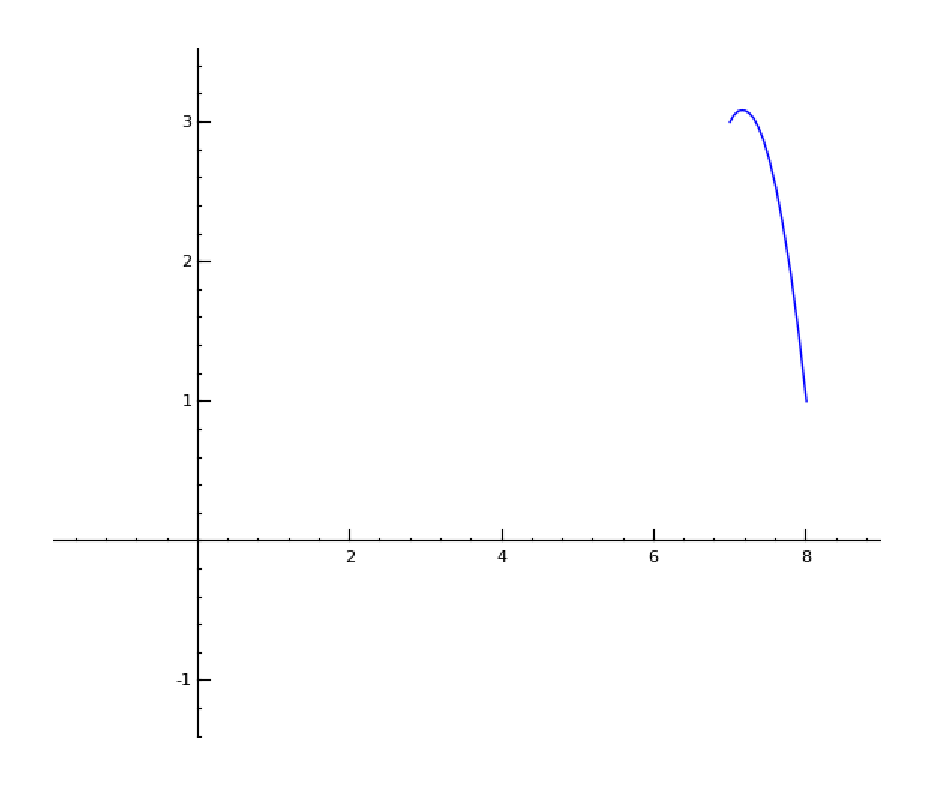
\includegraphics[height=5cm,width=7cm]{exercise-11-5-16.eps}
\end{center}
\end{minipage}
\caption{Plot for Exercise 11.5-16, $x=7+t^2$, $y =3 + t^2 - 3t^4$.}
\label{fig:exercise-11-5-16}
\end{figure}


\item
%17
$x = \cot\, t$, $y = \sin^3t$. 	

Ans. 
$\frac{dy}{dx} = -3 \sin^4 t \cos t$, 
$\frac{d^2 y}{dx^2} = 3 \sin^5 t (4 - 5 \sin^2 t)$.

\item
%18
$x = a(\cos\, t + \sin\, t)$, $y = a(\sin\, t - t\cos\, t)$. 	

Ans. $\frac{dy}{dx} = \tan t$, $\frac{d^2 y}{dx^2} = \frac{1}{at \cos^3 t}$.

\item
%19
$x = \frac{1 - t}{1 + t}$, $y = \frac{2t}{1 + t}$.

\item
%20
$x = 2t$, $y = 2 - t^2$.

\item
%21
$x = 1 - t^2$, $y = t^3$.

\item
%22
$x = a\cos\, t$, $y = b\sin\, t$.

\item
%23
Transform 
$\frac{ x \frac{dy}{dx} - y}{ \sqrt{1 
+ \left( \frac{dy}{dx} \right)^2} }$ by assuming 
$x = \rho \cos\theta$, $y = \rho \sin\theta$.

Ans. $\frac{\rho^2}{ \sqrt{ \rho \left( \frac{d\rho}{d\theta} \right)^2 } }$.

\item
%24
Let $f(x,y) = 0$ be the equation of a curve. Find an expression for 
its slope $\left( \frac{dy}{dx} \right)$ in terms of polar coordinates.

Ans. 
$\frac{dy}{dx} = \frac{ \rho \cos \theta 
+ \sin \theta \frac{d\rho}{d\theta} }{ -\rho \sin \theta 
+ \cos \theta \frac{d\rho}{d\theta} }$.

\end{enumerate}
